% Section 3: Problem Background

\section{Problem Background}

For the present context it is sufficient to restrict ourselves to optimal transport on $\mathbb {R}^d$. Let $X$,  $Y$ be subsets of $\mathbb{R}^d$ and let $\mu$ and $\nu$ be probability measures on $X$ and $Y$, respectively. In this paper we will always have X = Y , but using different notation for domain and target space makes definitions easier to grasp.

Transport map $T$ is any (measurable) map $X  \rightarrow Y$ that transforms the measure $\mu$ into the measure $\nu$. More precisely it satisfies $\mu(T^{-1}(B)) = \nu(B)$ for every measurable $B \subset Y$ . A transference plan is a measure $\pi$ on $X \times Y$ with marginals $\pi(\cdot \times Y) = \mu$ and $\pi(X \times \cdot) = \nu$. The set of transference plans from $\mu$ to $\nu$ is denoted by $\Pi(\mu, \nu)$. Any transport map $T$ from $\mu$ to $\nu$ defines a transference plan $\pi_T$ from $\mu$ to $\nu$ as the unique measure satisfying $\pi_{T}(A \times B)=\mu\left(A \cap T^{-1}(B)\right)$ for all measurable $A \subset X$ and $B \subset Y$. Not every transference plan $\pi$ can be represented in this way, because transference plans allow mass from one site $x \in X$ to be split between multiple destinations, which is not possible under a transport map. Figure 1 shows such an example.

\begin{figure}[htbp]
  \centering
  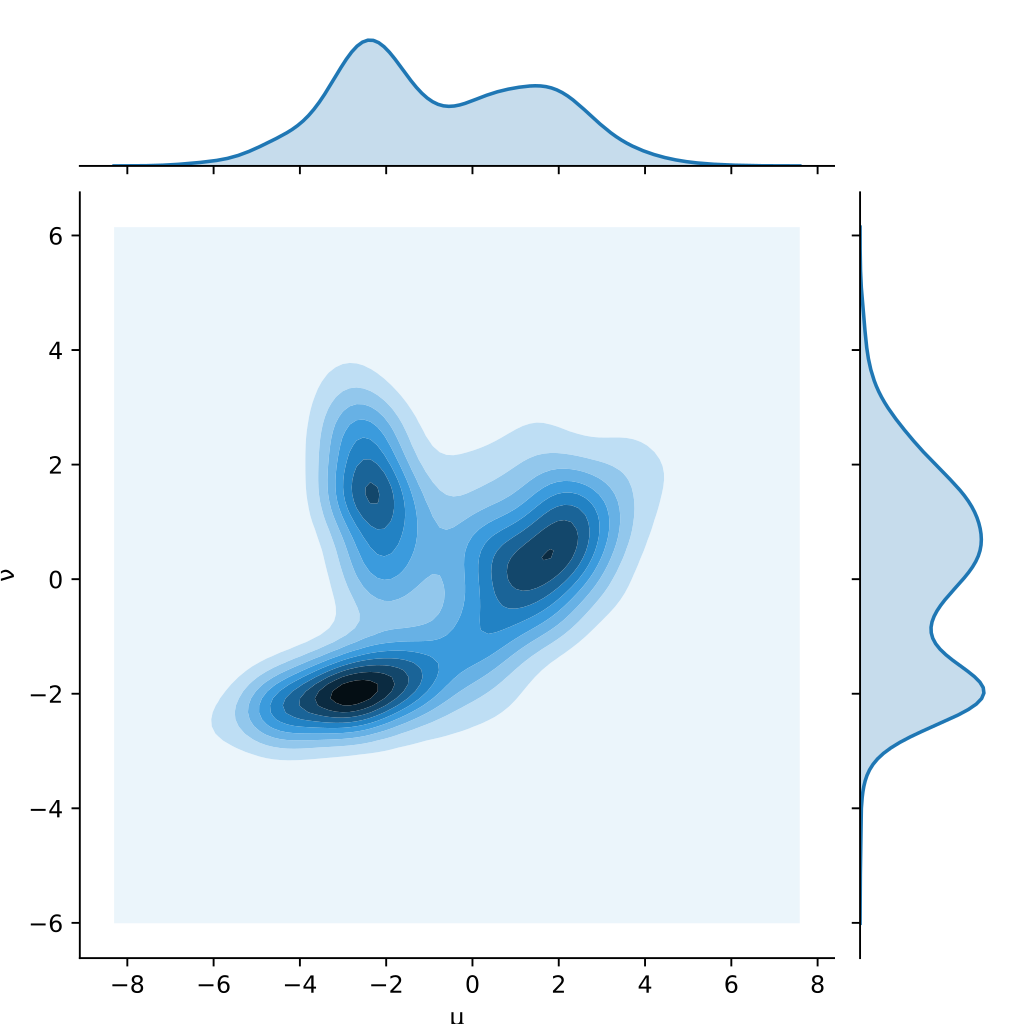
\includegraphics[width=0.8\linewidth]{img/1d_ot}
  \label{fig:ot}
  \caption{Two one-dimensional distributions $\mu$  and $\nu$ , plotted on the x and y axes, and one possible joint distribution that defines a transport plan between them.}
\end{figure}

We assume that the cost of transporting a unit mass from $x \in X$ to $y \in Y$ is $c_p(x,y) = \|x-y\|^p$ for some $p \geq 1$. The minimum cost for transferring $\mu$ to $\nu$ is then given by 

\begin{equation}
  C_p (\mu, \nu) = \min_{x \in \Pi(\mu,\nu)} \|x-y\|^p d\pi(x,y)
\end{equation}

Taking the $p^{th}$ root, we obtain the Wasserstein metric $W_p$. More precisely we have 

\begin{equation}
  W_p(\mu, \nu) = C_p(\mu, \nu)^{1/p}
\end{equation}

for and measures $\mu$ and $\nu$ that satisfy $\int_{X}\|x\|^{p} d \mu(x)<\infty$ adn $\int_{Y}\|y\|^{p} d \nu(y)<\infty$. In order to evaluate the Wasserstein metric, we need to find an optimal solution to $C_p(\mu,\nu)$, i.e., a minimizing transference plan $\pi$. This problem is often referred to as the Kantorovich formulation of optimal transport. Note that by Theorem 4.1 in [29] a minimizing always exists. However, it neither has to be unique nor representable in terms of an optimal transport map.

Often one would like to compare data sets that are available as images from a certain source, e.g. real photography, astronomical imagery, or microscopy data. We may think of such images as discrete measures on a grid. For example, tiny clippings from STED microscopy images of mitochondrial networks. A question of interest might be whether both images stem from the same part of the network, which can in principle be answered by finding an optimal transference plan (third panel in Figure 1) and computing the Wasserstein distance. Note that this coarse resolution is not representative for a serious analysis, but was only chosen for illustrative purposes.

Assume now that we have discrete measures of the form $\mu = \sum_{i=1}^m \mu_i \delta_{x_i}$ and $\nu = \sum_{j = 1}^n \nu_i \delta_{y_j}$ and write $c_{ij} = ||x_i - y_j||^p$. In what follows, we always have $m = n$, and $(x_i)_{1 \leq i \leq m} = (y_j)_{i\leq j \leq n}$ form a regular square grid in $R^2$, but since it is more intuitive, we keep different notation for source locations and target locations. Let $\pi_{ij}$ be the amount of mass transported from $x_i$ to $y_j$. Then, the problem can be rewritten as a linear program: 

\begin{equation}
  \begin{array}{rl}{\mathrm{(primal)}} & {\min_\pi \sum_{i=1}^{m} \sum_{j=1}^{n} c_{i j} \pi_{i j}} \\{\text { subject to }} & {\sum_{j=1}^{n} \pi_{i j}=\mu_{i},\quad \forall i=1, \ldots, m} \\{} & {\sum_{i=1}^{m} \pi_{i j}=\nu_{j},\quad \forall j=1, \ldots, n} \\{} & {\pi_{i j} \geq 0}\end{array}
\end{equation}

Note that this primal form has $mn$ variables which leads to computational difficulties, we can deduct the dual form of this problem as:

\begin{equation}
  \begin{array}{rl}{\mathrm{(dual)}} & {\max _{u, v} \sum_{i=1}^{m} \mu_{i} u_{i}+\sum_{j=1}^{n} \nu_{j} v_{j}} \\{\text { subject to }} & {c_{ij} - u_i - v_j \geq 0\qquad\forall i=1, \ldots, m \quad j = 1,\cdots,n}\end{array}
\end{equation}

Though only $m + n$ variables left, there still exist $mn$ constraints.